\chapter{Pickup Project}
\label{pickup-project}

After some studies it was decided to assembly a hexaphonic pickup instead buy one
already manufactured, which is an expansive device. To reduce the cost of the
project it was projected and printed the pickup base on 3D printer as the
project showed on figure 1.

\begin{figure}[!htpb]
\centering
\caption{3D pickup base project}
\label{3D-project}
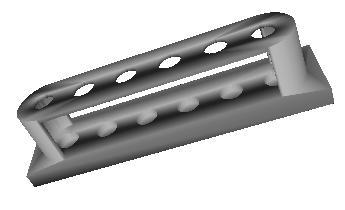
\includegraphics[scale=0.5]{images/Capt}
\legend{Source: made by authors}
\end{figure}

After print the pickup base it was assembled the coils, composed by guitar magnets
and copper iron (150 revolutions for each magnet), responsible for the transformation
of the mechanic vibration of the string to the electric signal which is needed.

\begin{figure}[!htpb]
\centering
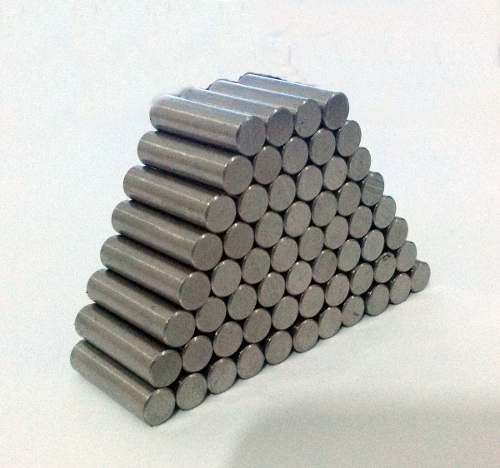
\includegraphics[scale=0.3]{images/ima}
\caption{Magnets}
\end{figure}

With the pickup already assembled it was verified the output signal. This signal
pick was about 0.5 mV and ths value was so weak to send to the Analogic-digital
converter present on the microprocessor. With this dungeon it was verified that
it is needed a circuit responsible for the signal amplification to be possible to
read the signal with quality on the microprocessor.
